\chapter{Mercoledì 01/04/2020}
\section{Esercitazione su progettazione}
\small
\subsection{Fasi del progetto}
Ricapitoliamo le varie fasi introdotte nella lezione precedente
\begin{itemize}
	\item \textbf{Analisi dettagliata delle specifiche fornite dal committente}\\ Questa fase è fondamentale per capire a fondo quali informazioni devono essere mantenute all’interno della base di dati. Scoprire in fase avanzata di progettazione che devono essere aggiunte nuove informazioni alla base di dati può essere molto costoso
	\item \textbf{Progettazione concettuale della base di dati}\\  Questa fase va dall’individuazione delle entità e delle relazioni, durante l’analisi delle specifiche, alla creazione dello schema concettuale (schema EntityRelationship)
	\item \textbf{Progettazione logica della base di dati}\\ Questa fase prende in pasto lo schema concettuale prodotto dalle fasi precedenti, e produce seguendo regole precise che richiedono poche scelte ulteriori lo schema logico (tabelle). 
	\item \textbf{Specifica dei vincoli}\\ Durante questa fase vengono specificati sia i vincoli di integrità referenziale (che derivano dalla traduzione in schema logico prodotta durante la fase precedente) che altri vincoli (necessari per mantenere la base di dati in uno stato consistente).
	\item \textbf{Realizzazione delle query}\\ Durante questa fase vengono create le query SQL che possono essere utilizzate per svolgere sulla base di dati le operazioni predefinite. 
\end{itemize}
\subsection{Specifiche di progetto}
\begin{itemize}
	\item Vogliamo progettare il sistema informativo di supporto ad un sito per l’acquisto di prodotti on-line. 
	\item Il sito potrà essere utilizzato solamente da utenti registrati, quindi anche gli acquisti possono essere effettuati solamente da utenti che si sono preventivamente registrati sul sito. Ovviamente è possibile che un utente sia registrato sul sito senza aver mai effettuato nessun acquisto. 
	\item I fornitori possono vendere i propri prodotti tramite il sito solo nel caso in cui siano preventivamente registrati. 
	\item I prodotti acquistati mediante il sito possono essere consegnati all’acquirente solamente da corrieri che siano preventivamente registrati sul sito.
	\item I fornitori offrono i propri prodotti, specificando prezzi e condizioni di vendita e di spedizione. 
	\item Uno stesso prodotto potrà essere venduto da fornitori diversi con prezzi e condizioni di vendita e spedizione diverse. 
	\item Il cliente sceglierà il fornitore da cui comprare un prodotto in base al suo criterio di scelta (a causa del prezzo, delle condizioni di vendita, ecc).
	\item Ciascun corriere metterà a disposizione della clientela vari tipi d consegna. 
	\item Ciascun fornitore registrato sul sito effettuerà accordi commerciali con alcuni dei corrieri registrati sul sito. 
	\item Nel momento in cui un fornitore decida di servirsi di un dato corriere, questi permetterà l’utilizzo di tutti i tipi di consegna messi a disposizione. 
	\item Nel momento in cui un cliente fa un ordine ad un fornitore potrà scegliere per la consegna solamente uno dei corrieri convenzionati con il fornitore. Ovviamente il cliente sceglierà il corriere in base a propri criteri (prezzo, tempi di consegna, garanzie offerte sulla consegna, ecc).
	\item Il sistema informativo dovrà mantenere anche informazioni sull’abbinamento di prodotti appartenenti a categorie diverse
	\begin{itemize}
		\item Ad esempio, se un cliente acquista un prodotto di categoria X, il sistema informativo dovrà essere in grado di consigliare i prodotti della categoria Y che sono abbinabili con il prodotto appena acquistato.
	\end{itemize}
	\item Nel caso in cui il cliente effettui un ordine tramite il sito potrà specificare il proprio grado di soddisfazione sull’operato del fornitore, inserendo nella base di dati un voto compreso tra 0 e 10. 
	\item Analogamente il cliente potrà specificare il proprio grado di soddisfazione sull’operato del corriere.
	\item Il voto che un cliente dà ad un fornitore o ad un corriere è legato ad un ordine e quindi ad una data.
	\item Sulla base di dati progettata dovranno essere effettuate delle query in grado di recuperare almeno le seguenti informazioni:
	\begin{itemize}
		\item Elenco di tutti i prodotti di una data categoria X che sono consigliati in seguito all’acquisto di un dato prodotto di categoria Y.
		\item Elenco dei fornitori che vendono il maggior numero di prodotti diversi di una data categoria X.
		\item Elenco dei fornitori che vendono un dato prodotto x a prezzo più basso.
		\item Elenco dei fornitori con voto medio più alto tra quelli che hanno un dato prodotto x presente in magazzino.
	\end{itemize}
	\item Inoltre sulla base di dati dovranno essere effettuate le seguenti operazioni:
	\begin{itemize}
		\item Inserimento di un nuovo ordine (con grado di soddisfazione del cliente nei confronti dell’operato del fornitore e del corriere nullo).
		\item Inserimento del grado di soddisfazione del cliente nei confronti dell’operato del fornitore e/o del corriere relativamente ad un ordine già effettuato.
		\item Inserimento di un nuovo prodotto nel magazzino di un fornitore (supponendo che tale prodotto fosse già presente all’interno della base di dati).
	\end{itemize}
\end{itemize}
\subsection{Individuazione entità}
\begin{itemize}
	\item Iniziamo la progettazione individuando le entità della base di dati:
	\begin{itemize}
		\item Gli Utenti sono registrati e costituiscono un’entità
		\item Un Prodotto è un’entità, la Categoria a cui appartiene può essere considerata come suo attributo
		\item La Spedizione (il tipo)
	\end{itemize}
	\item Possiamo specializzare Utente con Cliente, Fornitore e Corriere
	\item Otteniamo, quindi, la seguente situazione dove gli attributi in comune (Telefono, Indirizzo, e-mail, ecc) di Cliente, Fornitore e Corriere saranno attributi di
	Utente.
\end{itemize}
\begin{center}
	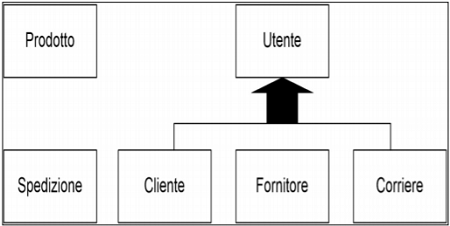
\includegraphics{images/86.PNG}
\end{center}
\begin{itemize}
	\item La base di dati deve tenere memoria degli ordini effettuati in modo che un voto possa essere assegnato sia ai fornitori che ai corrieri.
	\item Ciascun ordine consisterà delle seguenti informazioni:
	\begin{itemize}
		\item Cliente che ha effettuato l’ordine
		\item Fornitore che ha ricevuto l’ordine
		\item Corriere utilizzato per la consegna dell’ordine
		\item Tipo di spedizione utilizzato per recapitare l’ordine
		\item Prodotti acquistati tramite l’ordine
		\item Voto al corriere
		\item Voto al fornitore
	\end{itemize}
	\item Poiché un ordine non ha un’esistenza indipendente dalle altre entità (ad esempio un ordine non può esistere se non c’è un cliente che lo genera), possiamo classificare Ordine come una relazione.
	\item Ordine stabilisce un’associazione tra 5 entità diverse:
	\begin{itemize}
		\item Cliente
		\item Fornitore
		\item Corriere
		\item Spedizione
		\item Prodotti
	\end{itemize}
	\item Ed ha alcuni attributi propri: coto al corriere e voto al fornitore
	\item Nel ragionamento fin qui fatto abbiamo stabilito due punti che possono risultare difficili da gestire
	\begin{enumerate}
		\item una relazione connessa a 5 entità diverse pone problemi soprattutto per quanto riguarda l’individuazione delle cardinalità
		\begin{itemize}
			\item Possiamo pensare di raffinare (approccio topdown) la relazione Ordine in un’entità Ordine correlata alle 5 entità Cliente, Fornitore,.. da 5 relazioni diverse.
		\end{itemize}
		\item I prodotti hanno un attributo Categoria. Questa soluzione potrebbe dare origine a inconsistenze in fase di inserimento. Ad esempio, un fornitore potrebbe inserire
		\begin{itemize}
			\item Prodotto = “x”, Categoria = “RAM” 
			\item Prodotto = “y”, Categoria = “ram”
		\end{itemize}
		Come conseguenza nella base di dati i due prodotti risulterebbero appartenenti a categorie diverse
		\begin{itemize}
			\item Per evitare problemi di questo tipo possiamo effettuare ancora un raffinamento e trasformare Categoria in un’entità collegata a Prodotto da una relazione di appartenenza.
		\end{itemize}
	\end{enumerate}
	\item A questo punto lo schema delle entità risulterà il seguente: abbiamo una generalizzazione e alcune associazione già individuate
\end{itemize}
\begin{center}
	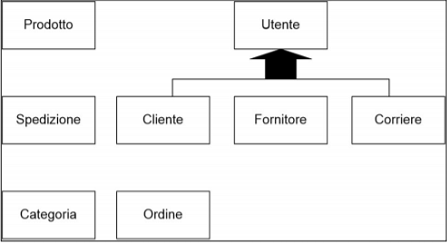
\includegraphics{images/87.PNG}
\end{center}
\subsection{Individuazione relazioni}
\begin{itemize}
	\item Occorre mettere in relazione l’entità Fornitore e l’entità Prodotto: introduciamo la relazione Vende
	\item Occorre mettere in relazione l’entità Fornitore e l’entità Corriere: introduciamo la relazione Accordo
	\item Occorre mettere in relazione l’entità Corriere e l’entità Spedizione: introduciamo la relazione Offre
	\item Occorre mettere in relazione l’entità Prodotto con se stessa per poter memorizzare l’abbinamento tra prodotti di categoria diversa: introduciamo la
	relazione Consiglia
\end{itemize}
\begin{center}
	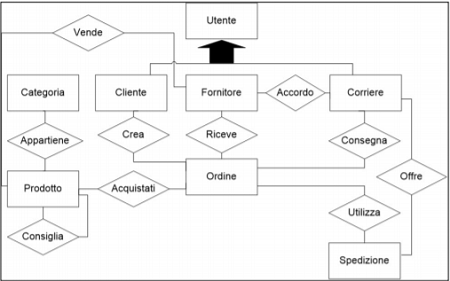
\includegraphics{images/88.PNG}
\end{center}
\subsection{Individuazione attributi}
\begin{itemize}
	\item Vediamo quali attributi associare alle varie entità: 
	\begin{itemize}
		\item Utente: Indirizzo, Telefono, E-mail,
		DataRegistrazione, UserName, Password
		\item Cliente: Nome, Cognome, CodFiscale
		\item Fornitore: RagSociale, PartitaIVA
		\item Corriere: RagioneSociale, PartitaIVA
		\item Categoria: CodCategoria, Descrizione \item Prodotto: CodProdotto, Marca, Modello, Descrizione, Foto
		\item Ordine: CodOrdine, DataEmissione, DataPagamento, TipoPagamento, DataConsegna, VotoFornitore, VotoCorriere
		\item Spedizione: AreaCoperta, DimMax, PesoMax
	\end{itemize}
	\item Non abbiamo associato il prezzo all’entità Prodotto perché un medesimo prodotto potrebbe essere venduto da fornitori diversi a prezzi diversi. 
	\item Analogamente non abbiamo associato il prezzo all’entità Spedizione perché supponiamo che uno stesso tipo si spedizione possa essere offerto da vari corrieri a prezzi diversi.
	\item Vediamo quali attributi potremmo associare alle varie relazioni:
	\begin{itemize}
		\item Vende: Prezzo, DispMagazzino
		\item Appartiene: nessun attributo
		\item Crea: nessun attributo
		\item Riceve: nessun attributo
		\item Acquistati: NumPezzi 
		\item Consiglia: nessun attributo
		\item Accordo: DataInizio, Durata
		\item Consegna: nessun attributo
		\item Utilizza: nessun attributo 
		\item Offre: Costo
	\end{itemize}
	\item Alla relazione Accordo abbiamo associato l’attributo DataInizio e Durata, ma supponiamo di non dover fare nessun controllo perché manterremo nella base di dati solamente gli accordi attualmente in vigore.
	\item Nella relazione Acquistati manteniamo memoria del numero di pezzi di ciascun prodotto richiesti in ciascun ordine
\end{itemize}
\begin{center}
	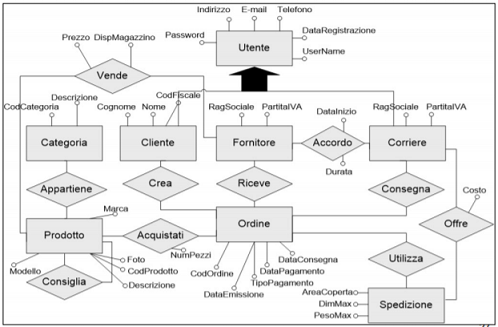
\includegraphics{images/89.PNG}
\end{center}
\subsection{Individuazione cardinalità}
\begin{itemize}
	\item Entità Ordine - Relazione Riceve: (1,1) in quanto un ordine viene ricevuto da un solo fornitore.
	\item Entità Ordine - Relazione Consegna: (1,1) in quanto un ordine viene recapitato da un solo corriere.
	\item Entità Ordine - Relazione Crea: (1,1) in quanto un ordine viene eseguito da un solo cliente.
	\item Entità Ordine - Relazione Utilizza: (1,1) in quanto per la consegna di un ordine si utilizza un solo tipo di spedizione.
	\item Entità Ordine - Relazione Acquistati: (1,N) in quanto un ordine può contenere più prodotti diversi.
	\item Entità Fornitore - Relazione Riceve: (0,N) in quanto un fornitore può aver ricevuto più ordini o nessun ordine (se ad esempio il fornitore si è appena iscritto al sito).
	\item Entità Fornitore - Relazione Accordo: (1,N) si suppone che, contemporaneamente all’iscrizione al sito, ogni fornitore si accordi con almeno un
	corriere.
	\item Entità Fornitore - Relazione Vende: (1,N) un fornitore può vendere più di un prodotto. Si suppone che, nel momento in cui si iscrive al sito, ogni fornitore sia in grado di vendere almeno un prodotto.
	\item Entità Corriere - Relazione Accordo: (0,N) un corriere può essere accordato con più fornitori o con nessun fornitore (ad esempio se si è appena iscritto al sito).
	\item Entità Corriere - Relazione Consegna: (0,N) un corriere può aver consegnato più ordini o nessun ordine (ad esempio se si è appena iscritto al sito).
	\item Entità Spedizione - Relazione Utilizza: (0,N) un tipo di spedizione può essere utilizzato per consegnare più ordini. È possibile però che un tipo di spedizione non sia mai stato utilizzato (ad esempio se è stato appena introdotto nel sito o se è particolarmente svantaggioso).
	\item Entità Spedizione - Relazione Offre: (1,N) un tipo di spedizione può essere offerto da più corrieri. Ciascun tipo di spedizione, però, deve essere offerto da almeno un corriere, altrimenti non avrebbe motivo di essere inserito nella base di dati del sito
	\item Entità Cliente - Relazione Ordine: (0,N) ciascun cliente può aver effettuato più ordini. È possibile che
	un cliente non abbia effettuato alcun ordine.
	\item Entità Prodotto - Relazione Vende: (1,N) un prodotto
	può essere venduto da più fornitori, e deve essere
	venduto da almeno un fornitore (altrimenti non
	avrebbe senso la presenza del prodotto nella base di
	dati del sito).
	\item Entità Corriere - Relazione Offre: (1,N) un corriere
	può offrire tipi di spedizione diversi. Si suppone che
	un corriere offra almeno un tipo di spedizione.
	\item Entità Prodotto - Relazione Consiglia: (1,N) ciascun
	prodotto ha almeno un altro prodotto consigliato.
	\item Entità Categoria - Relazione Appartiene: (1,N) la base
	di dati deve contenere almeno un prodotto per
	ciascuna categoria, infatti l’esistenza di una categoria
	vuota non avrebbe senso.
	\item Entità Prodotto - Relazione Appartiene: (1,1) ciascun
	prodotto appartiene ad una ed una sola categoria.
\end{itemize}
\begin{center}
	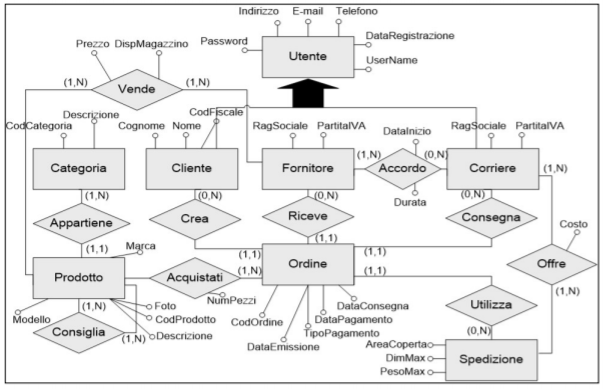
\includegraphics{images/90.PNG}
\end{center}
\subsection{Introduzione di nuovi attributi}
\begin{itemize}
	\item Se analizziamo le operazioni che devono essere compiute sulla base di dati ci rendiamo conto che potrebbe convenire introdurre dei nuovi attributi al fine di
	facilitarle. Questi attributi possono anche anche rappresentare informazione già presente nella base di dati.
	\item Consideriamo, ad esempio: elenco dei fornitori con voto medio più alto tra quelli che hanno un dato prodotto X presente in magazzino.
	\item In questo caso per recuperare il voto medio di un fornitore dobbiamo andare a leggere tutti gli ordini ricevuti da tale fornitore.
	\item Per facilitare questa operazione potremmo introdurre i seguenti attributi sull’entità Fornitore (perché non il voto medio direttamente?): TotaleVoti, NumeroVoti.
	\item In questo modo, ogni volta che introduciamo un ordine dovremo anche aggiornare questi attributi per il fornitore che ha ricevuto l’ordine.
	\item Quindi le operazioni coinvolte dall’introduzione di questi
	nuovi attributi sono le seguenti:
	\begin{itemize}
		\item Elenco dei fornitori con voto medio più alto tra quelli
		che hanno un dato prodotto x presente in magazzino.
		\item Inserimento del grado di soddisfazione del cliente
		nei confronti dell’operato del fornitore e/o del
		corriere in un ordine di cui si conosce il codice.
	\end{itemize}
	\item Per capire se l’introduzione dei nuovi attributi è
	vantaggiosa in termini di tempi di esecuzione, dobbiamo
	valutari i diversi costi per queste due operazioni.
\end{itemize}
\subsection{Riprendiamo le specifiche di progetto}
Al fine di prendere decisioni sulla struttura della base di dati, lo studente supponga che la base di dati
contenga:
\begin{itemize}
	\item 600 prodotti diversi
	\item 50 fornitori registrati
	\item 1500 clienti registrati
	\item 15 corrieri registrati
	\item 3 abbinamenti (in media) tra un prodotto x (di categoria X) e i prodotti della categoria Y.
	\item 5 ordini finora effettuati per ciascun prodotto.
\end{itemize}
\subsection{Tavola dei volumi}
\begin{itemize}
	\item Prima è necessario valutare il numero di istanze di una data entità o relazione. 
	\item Per fare questo dobbiamo basarci sulle indicazioni presenti all’interno delle specifiche. 
	\item Nel caso in cui queste non siano sufficienti, dovremo fare delle ulteriori ipotesi che faranno parte della descrizione finale della base di dati.\\
	\item Cliente: 1500 istanze (da specifiche) 
	\item Fornitore: 50 istanze (da specifiche) 
	\item Corriere: 15 istanze (da specifiche) 
	\item Utente: 1565 istanze (perché le persone che sono iscritte sia come clienti che come fornitori e/o corrieri
	hanno più di un account. Quindi gli utenti possono essere al più: 1565=1500+50+15) 
	\item Prodotto: 600 istanze (da specifiche) 
	\item Categoria: 30 istanze (supponiamo che la base di dati contenga 30 categorie diverse di prodotti) 
	\item Spedizione: 6 istanze (supponiamo che la base di dati contenga 6 tipi di spedizione diversi)
	\item Ordine: 3000 istanze (perché da specifiche vengono effettuati in media 5 ordini per ciascun prodotto: 3000=600*5) 
	\item Vende: 1800 istanze (supponiamo che ciascun fornitore venda in media 36 prodotti diversi: 1800=50*36) 
	\item Accordo: 150 istanze (supponiamo che ciascun fornitore si sia accordato in media con 3 corrieri diversi: 150=50*3) 
	\item Appartiene: 600 istanze (perchè ciascun prodotto appartiene ad una, ed una sola, categoria) 
	\item Crea: 3000 istanze (perché ciascun ordine è eseguito da un solo cliente) 
	\item Riceve: 3000 istanze (perché ciascun ordine è ricevuto da un solo fornitore)
	\item Consegna: 3000 istanze (perché ciascun ordine è recapitato da un solo corriere) 
	\item Utilizza: 3000 istanze (perché ciascun ordine è recapitato utilizzando un solo tipo di consegna) 
	\item Offre: 60 istanze (perché ciascun corriere offre in media 4 tipi di spedizione diversi: 60=15*4) 
	\item Acquistati: 6000 istanze (perché ciascun ordine comprende in media 2 prodotti diversi: 6000=3000*2) 
	\item Consiglia: 1800 istanze (perché da specifiche, ciascun prodotto ha in media 3 abbinamenti)
\end{itemize}
\subsection{Operazioni elementari}
\begin{itemize}
	\item Date le operazioni coinvolte
	\begin{itemize}
		\item Operazione 1: Elenco dei fornitori con voto medio più alto tra quelli che hanno un dato prodotto X presente in magazzino. 
		\item Operazione 2: Inserimento del grado di soddisfazione del cliente nei confronti dell’operato del fornitore e/o del corriere per un ordine di cui si conosce il codice. 
	\end{itemize}
	\item Dobbiamo individuare le operazioni elementari nei seguenti casi:
	\begin{itemize}
		\item svolgimento dell’operazione 1 senza nuovi attributi
		\item svolgimento dell’operazione 1 con nuovi attributi
		\item svolgimento dell’operazione 2 senza nuovi attributi
		\item svolgimento dell’operazione 2 con nuovi attributi
	\end{itemize}
	
	\item Esecuzione Operazione 1 senza attributi aggiuntivi:
	\begin{itemize}
		\item 1 lettura in Prodotto per recuperare il codice del prodotto
		\item 3 letture in Vende per recuperare il codice dei fornitori che vendono quel prodotto (un prodotto è venduto in media da 3 fornitori: 3=1800/600).
		\item 180 letture in Riceve per recuperare il codice degli ordini ricevuti dai fornitori che hanno quel prodotto
		in magazzino (ciascun fornitore riceve in media 60 ordini: 60=3000/50).
		\item 180 letture in Ordine per poter leggere il voto assegnato nei vari ordini ai fornitori che hanno quel prodotto in magazzino.
	\end{itemize}
	\item Esecuzione Operazione 1 con nuovi attributi:
	\begin{itemize}
		\item 1 lettura in Prodotto per recuperare il codice del
		prodotto
		\item 3 letture in Vende per recuperare il codice dei fornitori che vendono quel prodotto (un prodotto è venduto in media da 3 fornitori: 3=1800/600).
		\item 3 letture in Fornitore per recuperare il TotaleVoti e
		il NumeroVoti di ciascun fornitore che ha quel
		prodotto in magazzino.
	\end{itemize}
	\item Esecuzione Operazione 2 senza attributi aggiuntivi:
	\begin{itemize}
		\item 1 scrittura in Ordine per inserire un voto non nullo
	\end{itemize}
	\item Esecuzione Operazione 2 con attributi aggiuntivi:
	\begin{itemize}
		\item 1 scrittura in Ordine
		\item 1 lettura in Riceve per recuperare il fornitore che ha ricevuto l’ordine
		\item 1 lettura in Fornitore per recuperare il TotaleVoti e NumeroVoti
		\item 1 scrittura in Fornitore per scrivere il nuovo valore di TotaleVoti e NumeroVoti
	\end{itemize}
\end{itemize}
\subsubsection{Conclusioni}
\begin{itemize}
	\item Operazioni necessarie per svolgere l’operazione 1:\\363 letture $\to$ 363 operazioni elementari 
	\item Operazioni necessarie per svolgere l’operazione 1 con attributi aggiuntivi:\\ 6 letture $\to$ 6 operazioni elementari 
	\item Operazioni necessarie per svolgere l’operazione 2:\\ 1 scrittura $\to$ 2 operazioni elementari 
	\item Operazioni necessarie per svolgere l’operazione 2 con attributi aggiuntivi
	\begin{itemize}
		\item 2 scritture $\to$ 4 operazioni elementari
		\item 2 letture $\to$ 2 operazioni elementari
	\end{itemize}
	\item Supponendo che l’operazione 2 venga compiuta 10 volte più frequentemente rispetto all’operazione 1, avremo
	\begin{itemize}
		\item con i nuovi attributi:
		\begin{itemize}
			\item  6 Op. Elementari + 6*10 Op. Elementari 
			\item totale= 66 Op. Elementari
		\end{itemize}
		\item senza nuovi attributi:
		\begin{itemize}
			\item 363 Op. Elementari + 2*10 Op. Elementari 
			\item totale = 383 Op. Elementari
		\end{itemize}
	\end{itemize}
	\item Al fine di ridurre le operazioni elementari introduciamo i nuovi attributi all’interno dello schema ER.
\end{itemize}
\begin{center}
	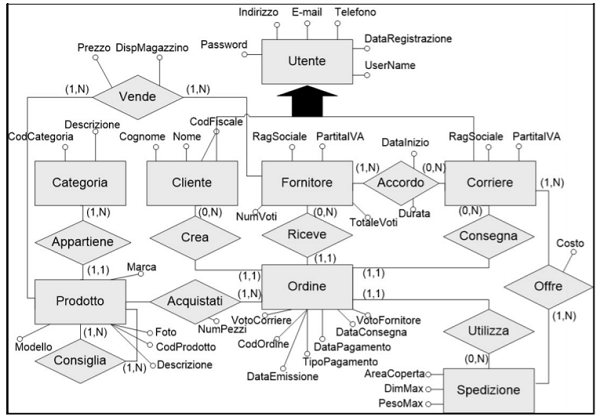
\includegraphics{images/98.PNG}
\end{center}
\subsection{Traduzione generalizzazioni}
\begin{itemize}
	\item Vediamo adesso come possiamo tradurre la generalizzazione presente nello schema ER. 
	\item Poiché si tratta di una generalizzazione totale, abbiamo tre possibilità:
	\begin{itemize}
		\item Lasciare padri e figli separati e collegarli utilizzando
		alcune relazioni.
		\item Accorpare l’entità padre sulle entità figlie
		\item Accorpare le entità figlie sull’entità padre. 
	\end{itemize}
	\item Analizziamo gli schemi ER che otteniamo in ciascuno di questi tre casi in modo da decidere quale di questi utilizzare.
\end{itemize}
\begin{center}
	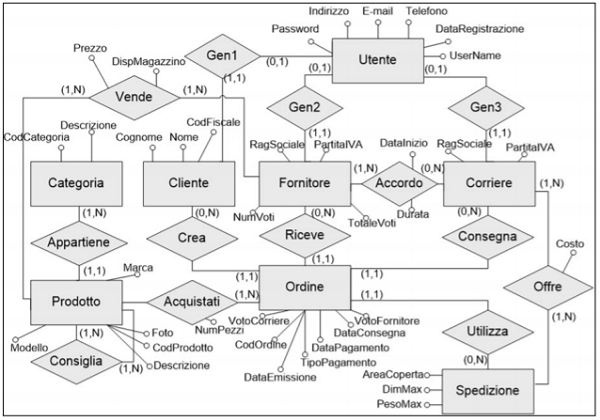
\includegraphics{images/97.PNG}
\end{center}
\begin{itemize}
	\item In questo modo abbiamo introdotto nello schema ER tre nuove relazioni. 
	\item Non abbiamo introdotto nessun valore NULL all’interno della base di dati.
	\item Abbiamo mantenuto un numero non troppo elevato di attributi per ciascuna entità
	\begin{itemize}\item quanto più il numero di attributi di un’entità è elevato, tanto più la gestione della relativa tabella diventa pesante. È quindi buona norma tentare di limitare il numero di attributi di ciascuna entità.\end{itemize}
\end{itemize}
\begin{center}
	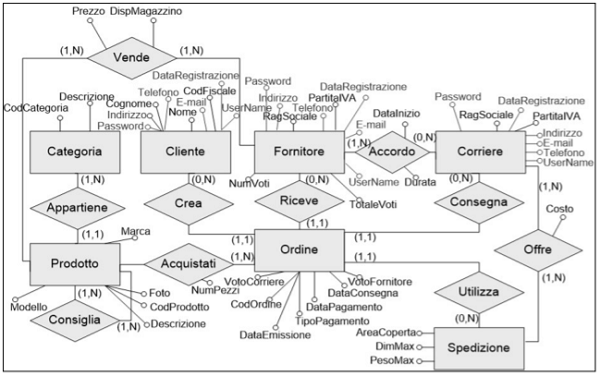
\includegraphics{images/96.PNG}
\end{center}
\begin{itemize}
	\item In questo modo non abbiamo introdotto nello schema
	nessuna nuova relazione. 
	\item Non abbiamo introdotto nessun valore NULL all’interno
	della base di dati. 
	\item Abbiamo però aggiunto alle entità Cliente, Fornitore e Corriere molti nuovi attributi (evidenziati in rosso nello schema ER) ottenendo tabelle più pesanti da gestire. 
	\item Inoltre, quando vogliamo controllare la correttezza di una coppia (username, password) dovremo controllare le coppie (username, password) presenti in tre diverse tabelle (a meno che non si sappia in anticipo se tale coppia appartiene ad un cliente, ad un fornitore o ad un corriere). 
\end{itemize}
\begin{center}
	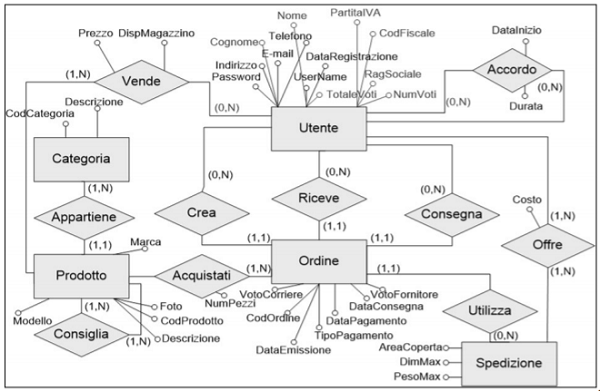
\includegraphics{images/95.PNG}
\end{center}
\begin{itemize}
	\item In questo modo non abbiamo introdotto nello schema ER
	nessuna nuova relazione. 
	\item Abbiamo però introdotto alcuni valori NULL all’interno dell’entità Utenti. 
	\item Il numero di attributi dell’entità Utenti è cresciuto
	molto. La tabella Utenti è molto pesante da gestire.
	\item Notare che anche se un fornitore vende
	necessariamente almeno un prodotto (cardinalità (1,N) tra la relazione Vende e l’entità Fornitori), non è detto
	che un utente (che può essere anche un cliente) venda necessariamente un prodotto (quindi cardinalità (0,N) tra la relazione Vende e l’entità Utenti). 
	\item Lo stesso vale per la relazione Accordo.\\
	
	\item Viste le tre possibili soluzioni, possiamo concludere che
	in questo caso conviene tradurre la generalizzazione
	lasciando l’entità padre e le entità figlie separate e
	collegate tramite relazioni. 
	\item In questo modo non introduciamo nessun valore NULL e
	il numero di attributi di ciascuna entità resta
	sufficientemente limitato. 
\end{itemize}
\begin{center}
	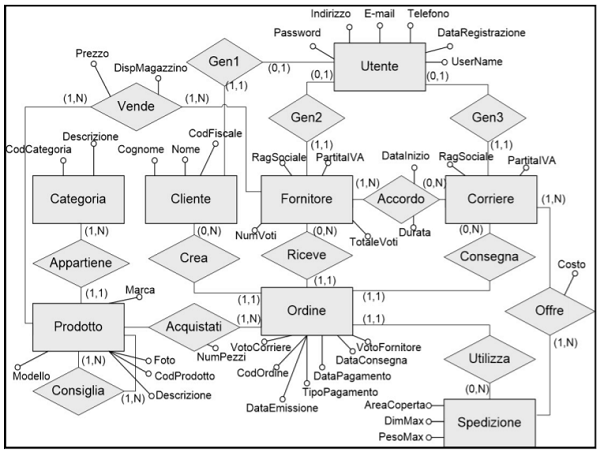
\includegraphics{images/94.PNG}
\end{center}
\subsection{Specifica chiavi}
Adesso dobbiamo specificare le chiavi delle varie entità:
\begin{itemize}
	\item Categoria: utilizziamo CodCategoria come chiave. 
	\item Prodotto: utilizziamo come chiave la coppia CodProdotto (attributo di prodotto) e CodCategoria
	(chiave dell’entità Categoria). 
	\item Ordine: utilizziamo CodOrdine come chiave. 
	\item Utente: utilizziamo UserName come chiave, in quanto ogni utente è caratterizzato dal proprio username. 
	\item Fornitore: potremmo utilizzare PartitaIVA come chiave, in quanto ogni fornitore è caratterizzato dalla propria partita IVA. In questo caso, peró, utilizzeremo come chiave lo UserName dell’utente associato.
	\item Corriere: potremmo utilizzare PartitaIVA come chiave, in quanto ogni corriere è caratterizzato dalla propria partita IVA. In questo caso, peró, utilizzeremo come chiave lo UserName dell’utente associato. 
	\item Cliente: potremmo utilizzare CodFiscale come chiave,
	in quanto ogni corriere è caratterizzato dal proprio codice fiscale. In questo caso, peró, utilizzeremo come chiave lo UserName dell’utente associato. 
	\item Spedizione: per identificare la spedizione dovremmo utilizzare gli attributi AreaCoperta, DimMax e PesoMax. Poiché utilizzare tre attributi come chiave
	può risultare scomodo, possiamo aggiungere un attributo CodSpedizione ed utilizzarlo come chiave.
\end{itemize}
\begin{center}
	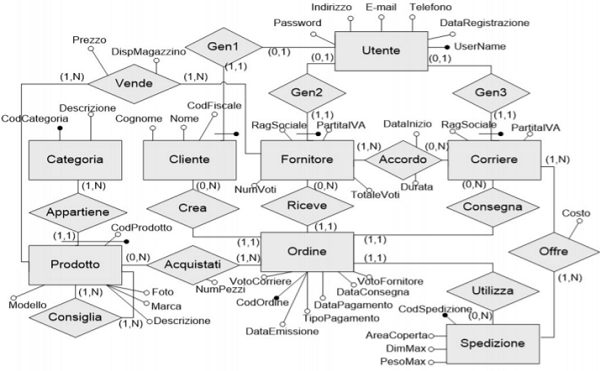
\includegraphics{images/93.PNG}
\end{center}
\subsection{Traduzione in tabelle}
\begin{itemize}
	\item Traduciamo lo schema ER ottenuto in tabelle
	\item Ciascuna entità viene tradotta in una tabella a se stante
	\item Vediamo come tradurre le varie relazioni:
	\begin{itemize}
		\item Gen1: la traduciamo accorpando la tabella sull’entitá Cliente (cardinalitá (1,1) tra la relazione Gen1 e
		l’entitá Clente) 
		\item Gen2: la traduciamo accorpando la tabella sull’entitá Fornitore (cardinalitá (1,1) tra la relazione Gen2 e
		l’entitá Fornitore) 
		\item Gen3: la traduciamo accorpando la tabella sull’entitá Corriere (cardinalitá (1,1) tra la relazione Gen3 e
		l’entitá Corriere) 
		\item Vende: la traduciamo in una tabella a sé stante (relazione da N a N)
		\item Accordo: la traduciamo in una tabella a sé stante (cardinalitá (1,N) tra la relazione Accordo e l’entitá Fornitore e cardinalitá (0,N) tra la relazione Accordo e l’entitá Corriere) 
		\item Appartiene: la traduciamo accorpando la tabella sull’entitá Prodotto (cardinalitá (1,1) tra la relazione Appartiene e l’entitá Prodotto) 
		\item Crea: la traduciamo accorpando la tabella sull’entitá Ordine (cardinalitá (1,1) tra la relazione Crea e
		l’entitá Ordine) 
		\item Riceve: la traduciamo accorpando la tabella sull’entitá Ordine (cardinalitá (1,1) tra la relazione Riceve e
		l’entitá Ordine) 
		\item Consegna: la traduciamo accorpando la tabella sull’entitá Ordine (cardinalitá (1,1) tra la relazione Consegna e l’entitá Ordine)
		\item Utilizza: la traduciamo accorpando la tabella
		sull’entitá Ordine (cardinalitá (1,1) tra la relazione
		Utilizza e l’entitá Ordine) 
		\item Acquistati: la traduciamo in una tabella a sé stante
		(cardinalitá (1,N) tra la relazione Acquistati e l’entitá
		Ordine e cardinalitá (0,N) tra la relazione Acquistati
		e l’entitá Prodotto) 
		\item Offre: la traduciamo in una tabella a sé stante
		(relazione da N a N) 
		\item Consiglia: la traduciamo in una tabella a sé stante
		(relazione da N a N)
	\end{itemize}
	\item Quindi otteniamo le seguenti tabelle:
	\begin{figure}[h]
		\begin{subfigure}{0.5\textwidth}
			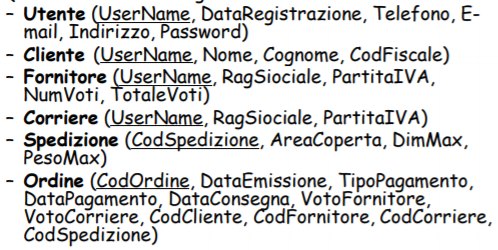
\includegraphics[width=0.9\linewidth]{images/91.PNG}
		\end{subfigure}
		\begin{subfigure}{0.5\textwidth}
			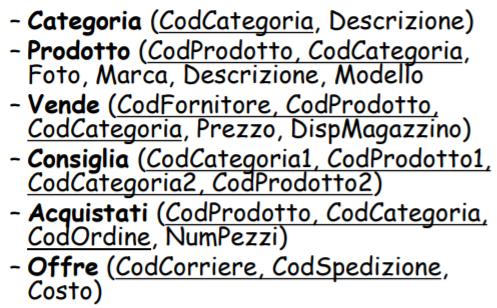
\includegraphics[width=0.9\linewidth]{images/92.PNG}
		\end{subfigure}
	\end{figure}
	
\end{itemize}
\subsection{Vincoli integritá referenziale}
Nel tradurre lo schema ER in tabelle, sono stati introdotti i seguenti vincoli di integritá referenziale:
\begin{itemize}
	\item  V.I.R.: tra l’attributo UserName della tabella Cliente
	e l’attributo UserName della tabella Utente.
	\item V.I.R.: tra l’attributo UserName della tabella
	Fornitore e l’attributo UserName della tabella
	Utente.
	\item V.I.R.: tra l’attributo UserName della tabella
	Corriere e l’attributo UserName della tabella Utente.
	\item V.I.R.: tra l’attributo CodCliente della tabella Ordine
	e l’attributo UserName della tabella Cliente.
	\item V.I.R.: tra l’attributo CodFornitore della tabella
	Ordine e l’attributo UserName della tabella
	Fornitore.
	\item V.I.R.: tra l’attributo CodCorrirere della tabella
	Ordine e l’attributo UserName della tabella Corriere
	\item V.I.R.: tra l’attributo CodSpedizione della tabella Ordine e l’attributo CodSpedizione della tabella Spedizione.
	\item V.I.R.: tra l’attributo CodCategoria della tabella Prodotto e l’attributo CodCategoria della tabella Categoria.
	\item V.I.R.: tra l’attributo CodCategoria della tabella Prodotto e l’attributo CodCategoria della tabella Categoria.
	\item V.I.R.: tra l’attributo CodFornitore della tabella
	Vende e l’attributo UserName della tabella Fornitore.
	\item V.I.R.: tra l’attributo CodProdotto della tabella Vende
	e l’attributo CodProdotto della tabella Prodotto.
	\item V.I.R.: tra l’attributo CodCategoria della tabella Vende e l’attributo CodCategoria della tabella Categoria.
	\item V.I.R.: tra l’attributo CodCategoria1 della tabella Consiglia e l’attributo CodCategoria della tabella Categoria.
	\item V.I.R.: tra l’attributo CodProdotto1 della
	tabella Consiglia e l’attributo CodProdotto della tabella Prodotto.
	\item V.I.R.: tra l’attributo CodCategoria2 della tabella Consiglia e l’attributo CodCategoria della tabella Categoria.
	\item V.I.R.: tra l’attributo CodProdotto2 della
	tabella Consiglia e l’attributo CodProdotto della tabella Prodotto.
	\item V.I.R.: tra l’attributo CodProdotto della
	tabella Acquistati e l’attributo CodProdotto della tabella Prodotto.
	\item V.I.R.: tra l’attributo CodCategoria della tabella Acquistati e l’attributo CodCategoria della tabella Categoria.
	\item V.I.R.: tra l’attributo CodOrdine della tabella
	Acquistati e l’attributo CodOrdine della tabella Ordine.
	\item V.I.R.: tra l’attributo CodCorriere della
	tabella Offre e l’attributo UserName della
	tabella Corriere.
	\item V.I.R.: tra l’attributo CodSpedizione della tabella Offre e l’attributo Cod Spedizione della tabella Spedizione.
\end{itemize}
\normalsize

\section{Implementazione dei vincoli}
L'algoritmo che ci permette l'uscita dallo schema E-R consiste in una serie di costrutti che permettono di creare le tabelle della nostra base di dati: le \emph{CREATE TABLE}.
\small
\begin{verbatim}
	CREATE TABLE Impiegato (
	Matricola CHAR(6) PRIMARY KEY,
	Nome CHAR(20) NOT NULL,
	Cognome CHAR(20) NOT NULL,
	Dipart CHAR(15),
	Stipendio NUMERIC(9) DEFAULT 0,
	FOREIGN KEY(Dipart) REFERENCES Dipartimento(NomeDip),
	UNIQUE(Cognome,Nome)
	)
\end{verbatim}
\normalsize
In questo caso abbiamo la relazione Impiegato, che presenta una serie di attributi. Ogni attributo è di un certo tipo e alcuni presentano delle clausole (\emph{keyword} associate agli attributi) per definire vincoli:
\begin{itemize}
	\item \textbf{Matricola} è la \emph{PRIMARY KEY}, ossia la chiave scelta per gli accessi dall'esterno. Segue che il valore dell'attributo non dovrà mai essere nullo e soprattutto essere unico, per permettere l'identificazione dei vari record. Il gestore verificherà che il valore indicato non sia già stato usato.
	\item \textbf{Nome} e \textbf{Cognome} sono \emph{NOT NULL}, cioè non possono essere mai vuoti.
	\item Con \emph{FOREIGN KEY} poniamo un vincolo di integrità referenziale. Si dice che l'attributo \textbf{Dipart} fa riferimento alla tabella Dipartimento, precisamente all'attributo \textbf{NomeDip}. Il valore indicato deve esistere come chiave nella tabella Dipartimento, altrimenti l'impiegato non viene inserito.
	\item Con \emph{UNIQUE} si stabilisce che non vi possono essere per forza aventi lo stesso \textbf{Nome} e \textbf{Cognome}.
\end{itemize}
\small
\begin{verbatim}
	CREATE TABLE Infrazioni(
	Codice CHAR(6) PRIMARY KEY,
	Data DATE NOT NULL,
	Vigile INTEGER NOT NULL REFERENCES Vigili(Matricola),
	Provincia CHAR(2),
	Numero CHAR(6),
	FOREIGN KEY(Provincia, Numero) 
	REFERENCES Auto(Provincia,Numero) ON DELETE SET NULL ON UPDATE CASCADE
	)	
\end{verbatim}
\normalsize
Qua abbiamo una tabella contenente le infrazioni. Ricordiamo quanto detto nella prima lezione: possiamo indicare il metodo per mantenere la consistenza della base di dati. Nell'esempio ho impostato la modifica del valore a NULL in caso di eliminazione e la modifica a cascata in caso di modifica.
\subsection{Vincoli di integrità generici: \emph{CHECK}}
Questi sono i vincoli basi garantiti al momento della tra duzione. Possiamo esprimere vincoli generici specificabili all'interno della tabella mediante la clausola \emph{CHECK}. Restringo i domini e specifico predicati (condizioni come quelle della clausola \emph{WHERE}) che devono essere soddisfatti ogni volta che un valore viene assegnato ad una variabile in quel dominio.
\begin{verbatim}
	CREATE TABLE Impiegato (
	Matricola CHARACTER(6),
	Cognome CHARACTER(20,
	Nome CHARACTER(20),
	Dipart CHARACTER(6),
	Ufficio CHARACTER(6),
	Sesso CHARACTER NOT NULL CHECK (Sesso IN('M','F')),
	Superiore CHARACTER(6),
	Stipendio INTEGER CHECK (Stipendio <= 
	(SELECT J.Stipendio FROM Impiegato AS J WHERE J.Matricola = Superiore)
	)
	)
\end{verbatim}
\begin{itemize}
	\item Voglio verificare che l'attributo \textbf{Sesso} assuma solo uno dei valori permessi (M, F)
	\item Voglio verificare che lo \textbf{Stipendio} dell'impiegato sia inferiore a quello del capo. Coinvolgo più attributi effettuando addirittura un'interrogazione.
\end{itemize}
La clausola CHECK può essere utilizzata all'interno della CREATE DOMAIN per stabilire un dominio.
\begin{verbatim}
	CREATE DOMAIN Voto 
	AS SMALLINT DEFAULT NULL
	CHECK (Value >= 18 AND Value <= 30)
\end{verbatim}
\subsubsection{ASSERTION}
Alcuni vincoli possono essere a livello non di un singola tabella ma di più tabelle. Attraverso un'asserzione, presente in una CREATE, stabilisco vincoli tra più tabelle.
\begin{verbatim}
	CREATE ASSERTION AlmenoUnImpiegato
	CHECK (1 <= (SELECT COUNT(*) FROM Impiegato))
\end{verbatim}
Con le asserzioni posso stabilire un qualunque vincolo predefinito: quando un'asserzione è stabilita ogni variazione del database è consentita solo se le asserzioni non vengono violate.
\subsubsection{Tipi di controllo} Si hanno due tipi di controllo
\begin{itemize}
	\item \textbf{Immediato}, verifica dopo ogni modifica
	\item \textbf{Differito}, verifica dopo una transazione (sequenza di operazioni)
\end{itemize}
Possiamo stabilire il tipo di controllo mediante il seguente costrutto
\begin{verbatim}
	SET CONSTRAINTS [NomeAss] (immediate | deferred)
\end{verbatim}
Un vincolo immediato non soddisfatto causa l'annullamento dell'operazione che ha causato la violazione (\emph{rollback parziale}), un vincolo differito non soddisfatto comporta l'annullamento di un'intera transazione (\emph{rollback}).
\paragraph{Nome delle asserzioni} Le asserzioni hanno un nome, quindi possono essere citate all'interno di istruzioni. Per esempio posso usare la seguente istruzione
\begin{verbatim}DROP NomeAss\end{verbatim} per eliminare l'asserzione con quel nome.
\subsection{Trigger}
Esiste un metodo diverso per inserire i vincoli, in un certo senso un vincolo dinamico. Esso reagisce in base a certi eventi avvenuti nel corso della computazione. Questi oggetti sono definiti \emph{trigger}.\\
Si stabiliscono delle condizioni che dovranno essere vere: se vere le istruzioni associate al trigger saranno eseguite. Abbiamo quindi i seguenti elementi:
\begin{itemize}
	\item \textbf{Evento} Solitamente si intendono modifiche dello stato del database: INSERT, DELETE, UPDATE. \\
	\small Se l'evento avviene il trigger è \emph{attivato} \normalsize
	\item \textbf{Condizione} La condizione che si deve verificare
	\small Se la condizione viene valutata il trigger è \emph{considerato} \normalsize
	\item \textbf{Azione} Ciò che viene eseguito con condizione vera
	\small Se l'azione è eseguita il trigger è \emph{eseguito} \normalsize
\end{itemize}
La sintassi dello standard attuale dell'SQL risale al 1999
\begin{verbatim}
	CREATE TRIGGER NomeTrigger
	{ BEFORE | AFTER } { INSERT | DELETE | UPDATE [of Column] } ON TabellaTarget
	[REFERENCING
	{[OLD TABLE [AS] VarTuplaOld] [NEW TABLE [AS] VarTuplaNew] } |
	{[OLD [ROW] [AS] VarTabellaOld] [NEW [ROW] [AS] VarTabellaNew] }
	]
	[FOR EACH { ROW | STATEMENT }]
	[WHEN Condizione]
\end{verbatim}
\subsubsection{Tipi di eventi}
\paragraph{BEFORE} Il trigger viene valutato prima della modifica dell'evento. Normalmente questa modalità è usata quando si vuole verificare una modifica prima che essa avvenga e "modificare la modifica"
\paragraph{AFTER} Prima si fa la modifica e successivamente si verificano le modifiche. Questa è la modalità più utilizzata.
\subsubsection{Granularità degli eventi}
\paragraph{Modalità di default \emph{statement-level}} Introdotta attraverso l'opzione \emph{for each statement}, il trigger viene considerato ed eseguito una volta sola per ogni statement che lo ha attivato, indipendentemente dal numero di tuple modificate.
\subsubsection{Conflitto tra trigger}
Se si hanno più trigger associati allo stesso evento possono emergere conflitti. Eseguo prima i BEFORE triggers e dopo la modifica gli AFTER triggers. Se i trigger appartengono alla stessa categoria l'ordine di esecuzione è stabilito in base alla data di creazione: i trigger più vecchi hanno priorità più alta.
\section{Istruzioni fondamentali per le transazioni}
\begin{itemize}
	\item BEGIN TRANSACTION: si specifica l'inizio di una transazione
	\item COMMIT WORK: la transazione è terminata con successo e quindi le operazioni specificate dopo la BEGIN TRANSACTION vengono eseguite sulla base di dati
	\item ROLLBACK WORK: si rinuncia all'esecuzione dell'operazioni specificate dopo la BEGIN TRANSACTION
\end{itemize}
\section{Integrazione con altri linguaggi di programmazione}
Abbiamo già visto che è possibile innesatare il linguaggio SQL con linguaggi di programmazione completamente diversi, per esempio il C++. Un precompilatore, legato al DBMS, viene usato per analizzare il programma e tradurlo in un programma nel linguaggio ospite (sostituendo le istruzioni SQL con chiamate alle funzioni di una API del DBMS). Tutto ciò avverrà ricorrendo a un'apposita libreria e dipenderà dal sistema operativo presente sulla macchina.
\paragraph{Attenzione} Il precompilatore è specifico per i linguaggi di programmazione coinvolti.
\paragraph{Conflitto di impedenza} Differenza tra ciò che può utilizzare un linguaggio di alto livello e ciò che SQL mette a disposizione. Il conflitto è risolto attraverso una tecnica detta \emph{cursore}: trasformiamo ciò che viene trasmesso dal DBMS, con il cursore scorriamo il buffer e leggiamo le tuple una alla volta. Successivamente il programma ricostituisce la struttura. Si ha una sorta di lettura da file dove il puntatore è appunto il cursore: si inizia un'operazione di lettura e alla fine si conclude con la chiusura del cursore.
\paragraph{SQL Statico ed SQL Dinamico} Le operazioni introdotte fino ad ora sono di tipo statico. Non sempre le istruzioni sono note quando scriviamo il programma! L'SQL dinamico permette la costruzione di istruzioni da parte del programma e non è banale gestire i risultati.\\
Un esempio si ha con la \emph{Call Level Interface}: si presuppone la presenza di un'interfaccia che chiede l'esecuzione di una certa operazione. Questo permette di interrogare un database anche con strutture diverse.
\paragraph{SQL Immerso VS CLI} La prima è più efficiente e permette l'esecuzione di tutte le funzioni di SQL. La CLI è indipendente, generica, permette di accedere a più basi, ma non fornisce tutte le funzionalità.